\section{Initial Results} \label{sec:evaluation}
We implemented the normal case of our protocol and collected initial 
results.

Evaluation was done on nine RDMA-enabled Dell R430 and five Supermirco 
SuperServer 1019P hosts. Each host has Linux 3.16.0 and 2.6 GHz Intel Xeon 
CPU. The Dell R430 hosts are equipped with 24 hyperthreading cores, 64 GB 
memory, and 1 TB SSD. The SuperServer 1019P hosts have 28 hyperthreading 
cores, 32 GB memory, and 375GB SSD. All NICs are Mellanox ConnectX-3 (40Gbps) 
connected with RoCE~\cite{roce}.

We compared \xxx with five open source consensus protocols, including four 
traditional ones (\libpaxos~\cite{libpaxos}, \zookeeper~\cite{zookeeper}, 
\crane~\cite{crane:sosp15} and \spaxos~\cite{spaxos:srds12}).

We evaluated \xxx on \nprog widely used or studied programs, including
\nkvprog key-value stores \redis, \memcached, \ssdb, \mongodb; \mysql, a SQL
server; \clamav, an anti-virus server that scans files and delete malicious 
ones; \mediatomb, a multimedia storage server that stores and transcodes video 
and audio files; \openldap, an LDAP server; \calvin~\cite{calvin:sigmod12}, a 
popular \smr system for databases.

\subsection{Comparing w/ Traditional Consensus}
\label{sec:eval-traditional}

\begin{figure}[t]
\begin{center}
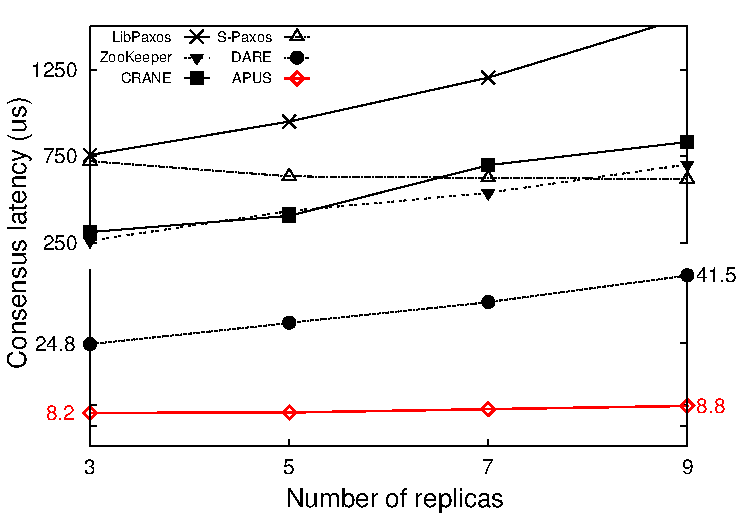
\includegraphics[width=3in]{figures/traditional_paxos_latency}
\caption{{\em Comparing \xxx to five existing consensus protocols.} All 
six protocols ran a client with 24 concurrent connections. The Y axis is 
broken to fit in all protocols.}
\label{fig:scalability}
\end{center}
\end{figure}

We ran \xxx and four traditional consensus protocols using their own 
client programs or popular client programs with 100K requests of similar sizes. 
For each protocol, we ran a client with 24 concurrent connections on a 24-core 
machine located in LAN, and we used up to nine replicas. Both the number of 
concurrent connections and replicas are common high 
values~\cite{zookeeper,crane:sosp15,rex:eurosys14,dare:hpdc15}.

Figure~\ref{fig:scalability} shows that the consensus latency of three 
traditional protocols increased almost linearly to the number of replicas 
(except \spaxos). \spaxos batches requests from replicas and invokes consensus 
when the batch is full. More replicas can take shorter time to form a batch, so 
\spaxos incurred a slightly better consensus latency with more replicas. 
Nevertheless, its latency was always over 600 \us. \xxx's consensus latency 
outperforms these four protocols by at least \comptradlow.

\subsection{Performance Overhead} \label{sec:overhead}

To stress \xxx, we used nine replicas to run all \nprog server 
programs without modifying them. We used up to 32 concurrent 
client connections (most evaluated programs reached peak throughput at 
16), and then we measured mean response time and throughput in 50 runs.

\begin{figure*}[t]
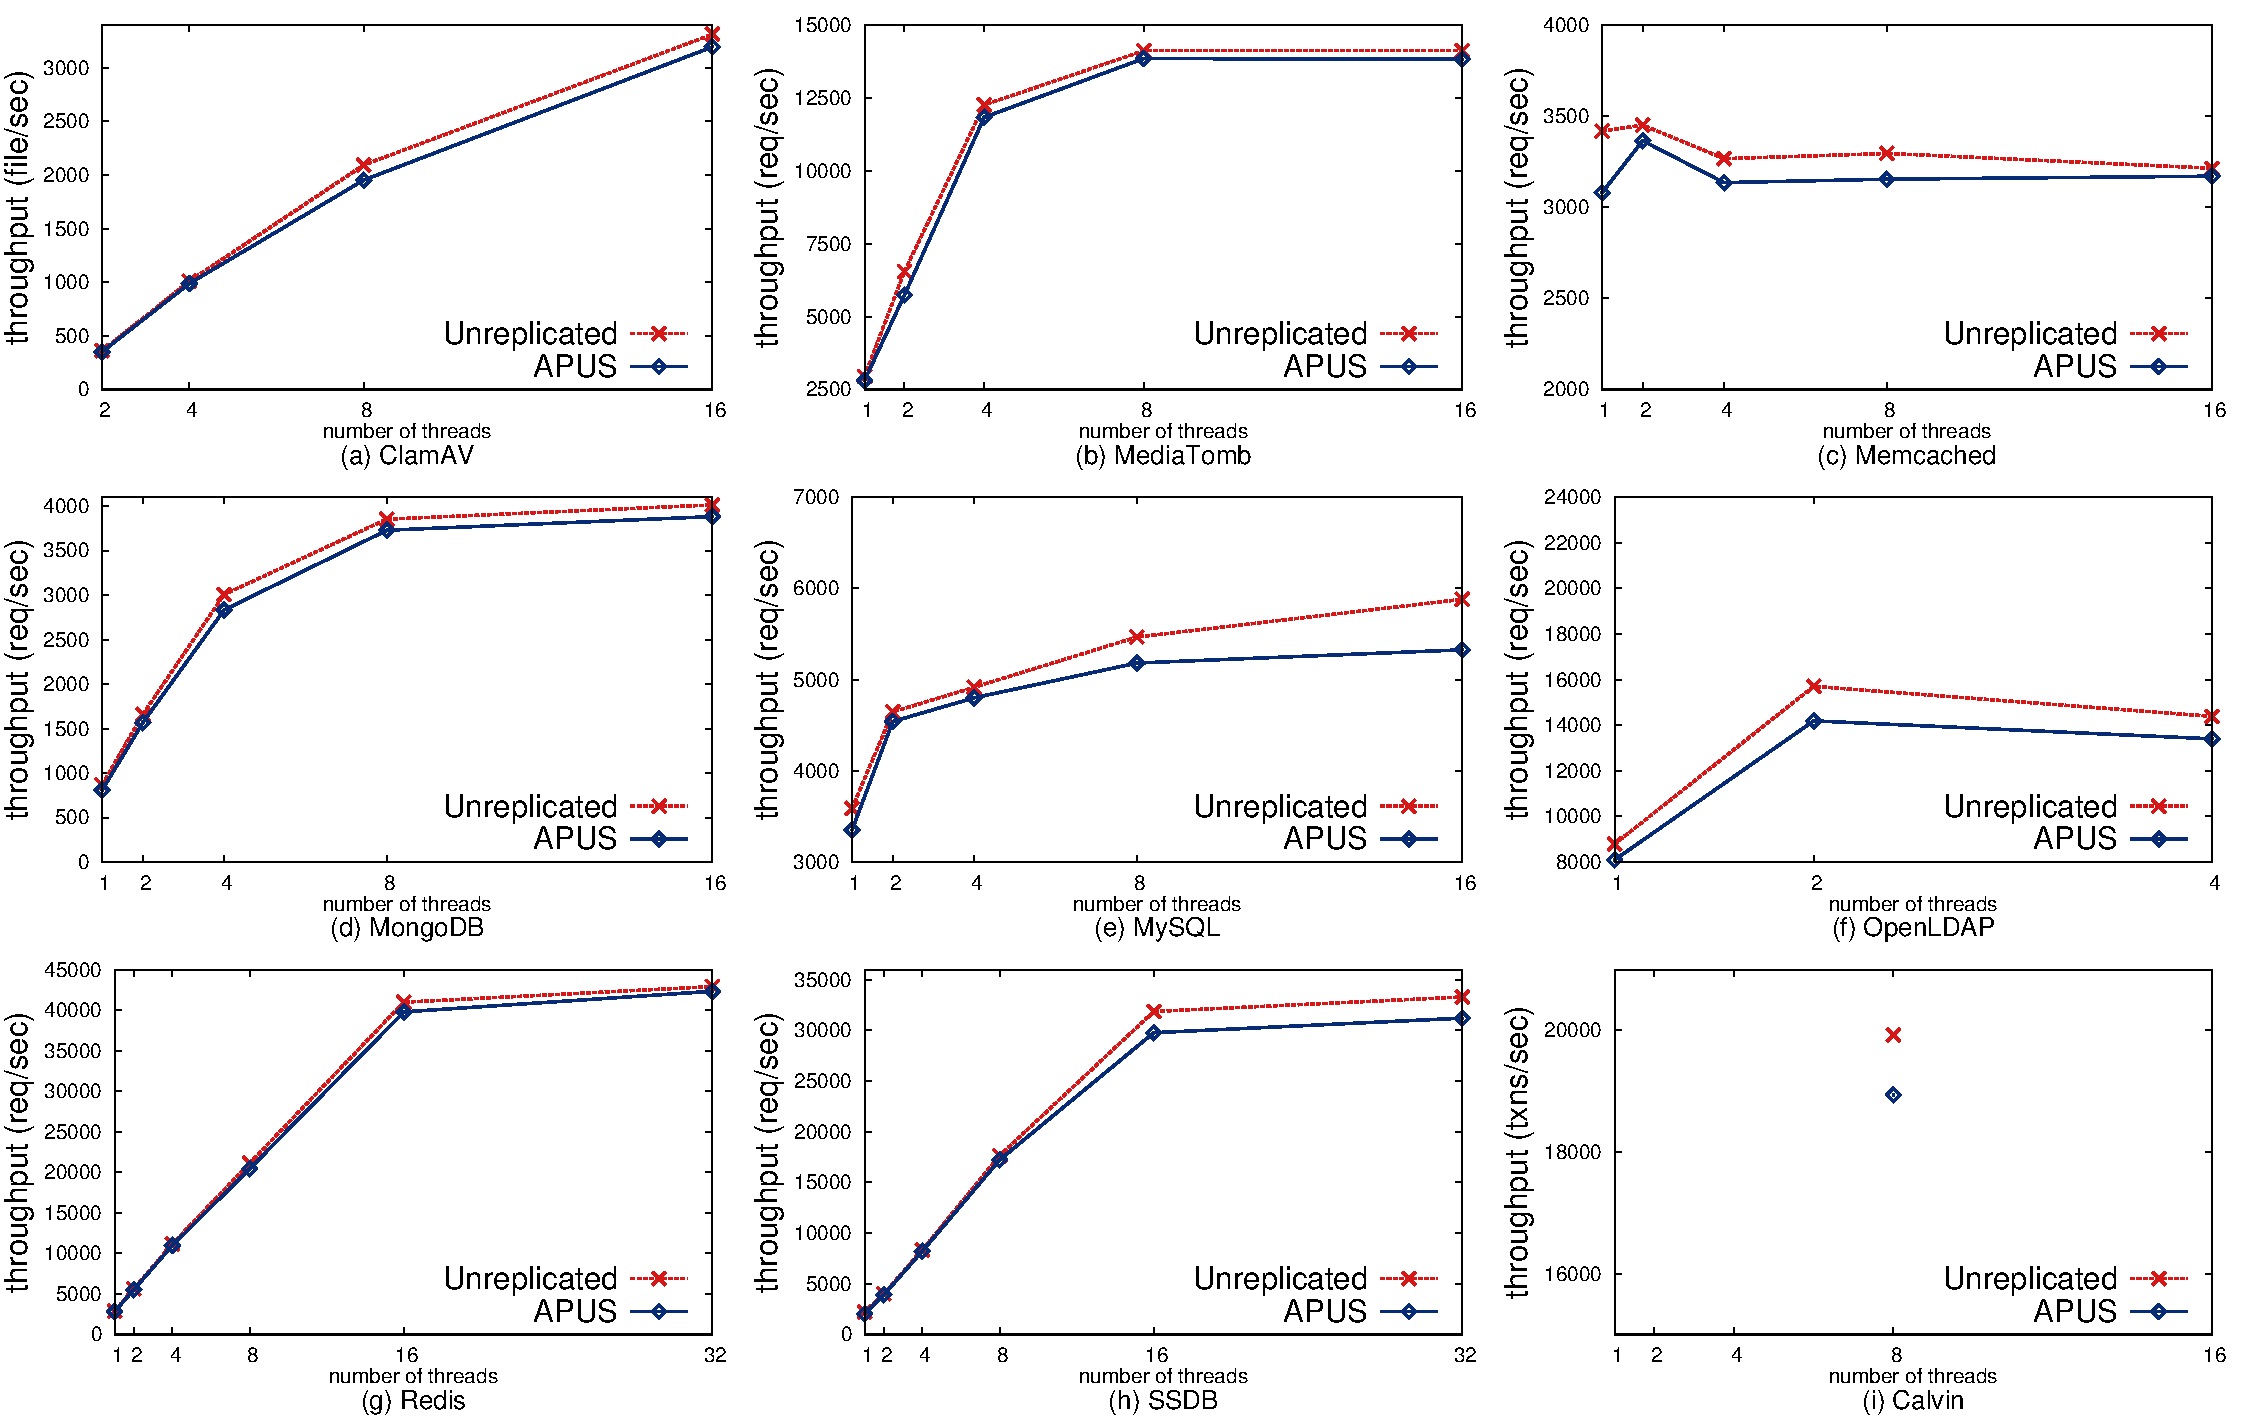
\includegraphics[width=6in]{figures/throughput}
\caption{\small {\em \xxx throughput compared to server programs' unreplicated
executions.}}
\label{fig:tput}
\end{figure*}

We turned on output checking and didn't 
observe a performance impact. Only two programs (\mysql and \openldap) 
have different output hashes caused by physical times 
(an approach~\cite{paxos:practical} can be leveraged to enforce same physical 
times across replicas).

Figure~\ref{fig:tput} shows \xxx's throughput. For \calvin, we only collected 
the 8-thread result because \calvin uses this constant thread count in their 
code to serve requests. Compared to these server programs' 
unreplicated executions, \xxx merely incurred a mean throughput overhead of 
\tputoverhead (note that in Figure~\ref{fig:tput}, the Y-axises of most 
programs start from a large number). As the number of threads increases, all 
programs' unreplicated executions got a performance improvement except 
\memcached. Prior work~\cite{rex:eurosys14} also showed that
\memcached itself scaled poorly. Overall, \xxx scaled as well as unreplicated 
executions on concurrent requests.

\subsection{Integrating \xxx into virtual machine} \label{sec:overhead}
Virtual machines usually use a primary-backup architecture for fault 
tolerance~\cite{alsberg1976principle}. However, primary-backup approach is 
notorious for the ``split-brain'' problem~\cite{scales2010design}, which can be 
avoided in \paxos. One reason for fault tolerant VMs to use 
primary-backup replication instead of \paxos protocol is that traditional \paxos 
systems incur high performance overhead. Specifically, every 
request received by the virtual machine must go through the traditional \paxos 
systems to reach consensus first, which takes hundreds of microseconds, and then 
be processed by the server programs. This high consensus latency severely 
degrades the performance of the applications running inside.

By integrating the fast \xxx \paxos protocol into virtual machine, we 
efficiently mitigate the ``split-brain'' problem caused by the primary-backup 
approach. We implemented the prototype on KVM QEMU hypervisor and it took fewer 
than ten lines of code by leveraging the simple API provided by \xxx.
